\chapter{Introducción}
\label{chap:introducción}

\emph{Estar preparado para la guerra\\ es uno de los medios más eficaces\\ para conservar la paz\\ George Washington}\\

En el siglo XXI toda pasa por ser digital y sino, ya es que lo era antes de llegar a este punto. Quizás muchas de las tecnologías que hoy conocemos se basen en un sistema informatizado, ya sea en su formato de software o sistema embebido. Y es que todo pasa por ser una herramienta software diseñadas para un propósito en concreto: un mecanismo de apertura de puertas mediante tarjetas rfid, procedimientos industriales o aplicados a alguna infraestructura crítica o de bien común, una aplicación del tiempo en tú terminal móvil, el propio sistema operativo con el que se puede leer el documento, etc. \\

Hay un sinfín de aplicaciones software que hacen nuestro día a día más llevadero y más fácil. Pero hay un punto que no todos conocen y es la necesidad de saber cómo se ha creado ese producto o cómo funciona realmente por su interior. En ése interior, a veces, podemos encontrar cosas que no estaban predestinadas a tener ese comportamiento y debido a ése comportamiento anómalo o imprevisto se generan situaciones de incertidumbre en las que el ser humano debe estar capacitao a afrontar. Dichas situaciones se suelen conocer con el término anglosajón de "bug" y sobre los bugs hay una especial categoría que se denominan fallas de seguridad o critical/several bugs. \\

Estas situaciones contractuales provocan que nuestro sistema, sea el que fuese, actúe de forma inesperada ante un input de información permitido o legítimo permitiendo un uso inadecuado de los recursos a los que se acceden mediante la aplicación. De este concepto o problema, surge en gran medida, el término de seguridad informática el cuál intenta abarcar y dar solución a estos problemas que pueden ir desde un simple fallo de desarrollo a un fallo crítico que comprometa la seguridad o confidencialidad de los documentos de una empresa o gobierno. \\

Debido a esta problemática, surge la necesidad de analizar, monitorizar y generar sistemas de seguridad perimetral que permita a las empresas ver que tipo de tráfico interno se genera, que tipo de tráfico externo tiene y cómo se hace uso de él (navegación hacia el exterior, tuneles vpn, conexiones remotas a dispositivos, etc). Así pues, se podría decir que para obtener este tipo de eventos sobre protocolos, tráfico, dns, ips, vpns,.. se tienen que configurar dispositivos de seguridad para la recolección de estos tipos de inputs o fuentes. \\

Una de las fuentes más conocidas dentro del mundo de la informática es el firewall, pero no así de las de un uso más extendido dentro del mundo doméstico sino el comercial o corporativo. Y dentro de los muchos tipos de softwares enfocados a tráfico (firewall) se encuentra el paquete de las distribuciones GNU/Linux iptables (software fruto del proyecto Netfilter para el kernel de GNU/Linux). Con esta herramienta se pueden definir políticas de filtrado de tráfico para cualquier tipo de protocolo tcp/udp que queramos limitar entre el exterior y nuestra máquina y viceversa. Además, estas políticas nos permiten derivar dicho tráfico a archivos que podemos manipular obteniendo así los eventos que representan al tráfico generado por una máquina conectada a una red, que posteriormente podemos manipular para generar estadísticas o tipos de uso para una red. \\

Aquí nace éste proyecto final de carrera. La solución que se busca desarrollar se denominaría Sensor de Seguridad (Security Sensor). De forma muy general, éste software se encargará de monitorización información de una máquina (logs, red (iptables), etc), almacenarla, visualizarla y además realizar un procesado de la misma con un algoritmo de obtención de características específico. \\

\section{Objetivos}

El objetivo principal del proyecto es controlar los tipos de conexiones entrantes y salientes de una máquina en sus diferentes protocolos de comunicación y mecanismos de gestión.

La aplicación deberá cumplir los siguientes requisitos:

\begin{itemize}
\item Ser una herramienta multiplataforma y que permita a cualquier usuario definir sus propias interfaces de gestión de eventos.
\item Dotar de funcionalidad gráfica que permita extraer información en tiempo real con gráficas o mecanismos visuales (en web) del sistema de base de datos que ha procesado los inputs de las fuentes para las que ha sido configurada.
\item Dotar de una api interna que nos permita extraer información en tiempo real en un formato uniforme para la web o para que cualquier usuario pueda usar la funcionalidad del proyecto para su propio beneficio usando herramientas generadas en el back-end para otro tipo de aplicaciones.
\item Ser parte de un todo, en el que el todo sea un SIEM capaz de obtener información de las diferentes sondas o módulos, que en este caso, sería la solución desarrollada.
\item Desarrollar una sonda para procesar eventos logs de firewall.
\end{itemize}

\section{Contexto: Seguridad informática}

La seguridad informática es el proceso de mantener un aceptable nivel de percepción frente a un riesgo. Así pues ninguna organización se puede considerar ``segura'' en cualquier momento, más allá de la última comprobación que se realizo dentro de su política de seguridad.

Un proceso seguro se encuadra dentro de las siguientes 4 etapas: Evaluación, Protección, Detección y Respuesta:

\begin{itemize}
\item Evaluación: es la preparación para las otras 3 etapas. Se considera cómo una acción separada porque se relaciona con las políticas, procedimientos, leyes, reglamentos, presupuestos y otras funciones de gestión, además de la propia evaluación técnica enfocada a la seguridad. No tener en consideración estos supuestos anteriores, podría dañar las etapas del diseño.
\item Protección: es la aplicación de contramedidas para reducir la probabilidad de tener una situación comprometida. La prevención es un término equivalente, pero cabe decir que en la mayoría de casos este concepto suele inducir al error (o al fallo).
\item Detección: es el proceso de identificación de intrusos. Una intrusión se puede considerar cómo una violación de una política de seguridad o cómo un incidente de seguridad a nivel de software/dispositivo.
\item Respuesta: es el proceso de validar los inputs recogidos por la detección para tomar medidas que solucionen las intrusiones. El primer enfoque que debemos realizar consiste en restaurar la funcionalidad dañada y seguir recopilando información para tener claras las evidencias del atacante sobre nuestro sistema y poder así emprender las acciones legales que correspondan.
\end{itemize}

\subsection{¿Qué es el riesgo?}

Cómo ya se mencionó en la definición de seguridad, el riesgo, es la posibilidad de sufrir un daño o pérdida. El riesgo, es una medida de peligro para un activo. Un activo se puede considerar cualquier cosa de valor, que en el contexto en el que nos encontramos se refiere a la información, hardware, propiedad intelectual, prestigio y reputación. Esto se puede definir cómo, ``riesgo de comprometer la integridad de la base de datos de un cliente'' o ``riesgo de una denegación de servicio al portal eléctronico de una entidad pública de gestión''. Se suele expresar en términos de una ecuación de riesgo, dónde:
$$ Riesgo\ =\ Amenaza\ \times\ Vulnerabilidad\ \times\ Valor\ del\ activo $$

\begin{itemize}
\item Amenaza: es el conjunto de las capacidades e intenciones de un atacante para explotar una vulnerabilidad en activo.
\item Vulnerabilidad: es una debilidad de un activo que podría conducir a la explotación del mismo. Las vulnerabilidades se introducen en los activos a través de un mal diseño, implementación o de contención de datos.
\item Valor del activo: es una medida de tiempo en relación a los recursos necesarios para reemplazar un activo o restaurarlo a su estado anterior funcional.
\end{itemize}

\section{Alcance}

El proyecto Security Sensor dará cómo resultado una aplicación software con interfaz visual web, que cumplirá con todos los objetivos y especificaciones indicados en el apartado anterior.

La aplicación se distinguirá en varias partes:
\begin{itemize}
\item Configuración y parametrización de los eventos logs de firewall en el dispositivo.
\item Recolección de logs mediante rsyslog y su posterior procesamiento.
\item Almacenaje en BD para su posterior manipulación interna o externa (api).
\item Extracción de características de los eventos y visualización de los mismos mediante un servicio web.
\item Aplicación de un algoritmo de procesamiento para comprimir la información en formato módulo para ser servida a un nodo central de gestión (SIEM).
\end{itemize}

\begin{figure}[H]
  \hspace*{0.65in}{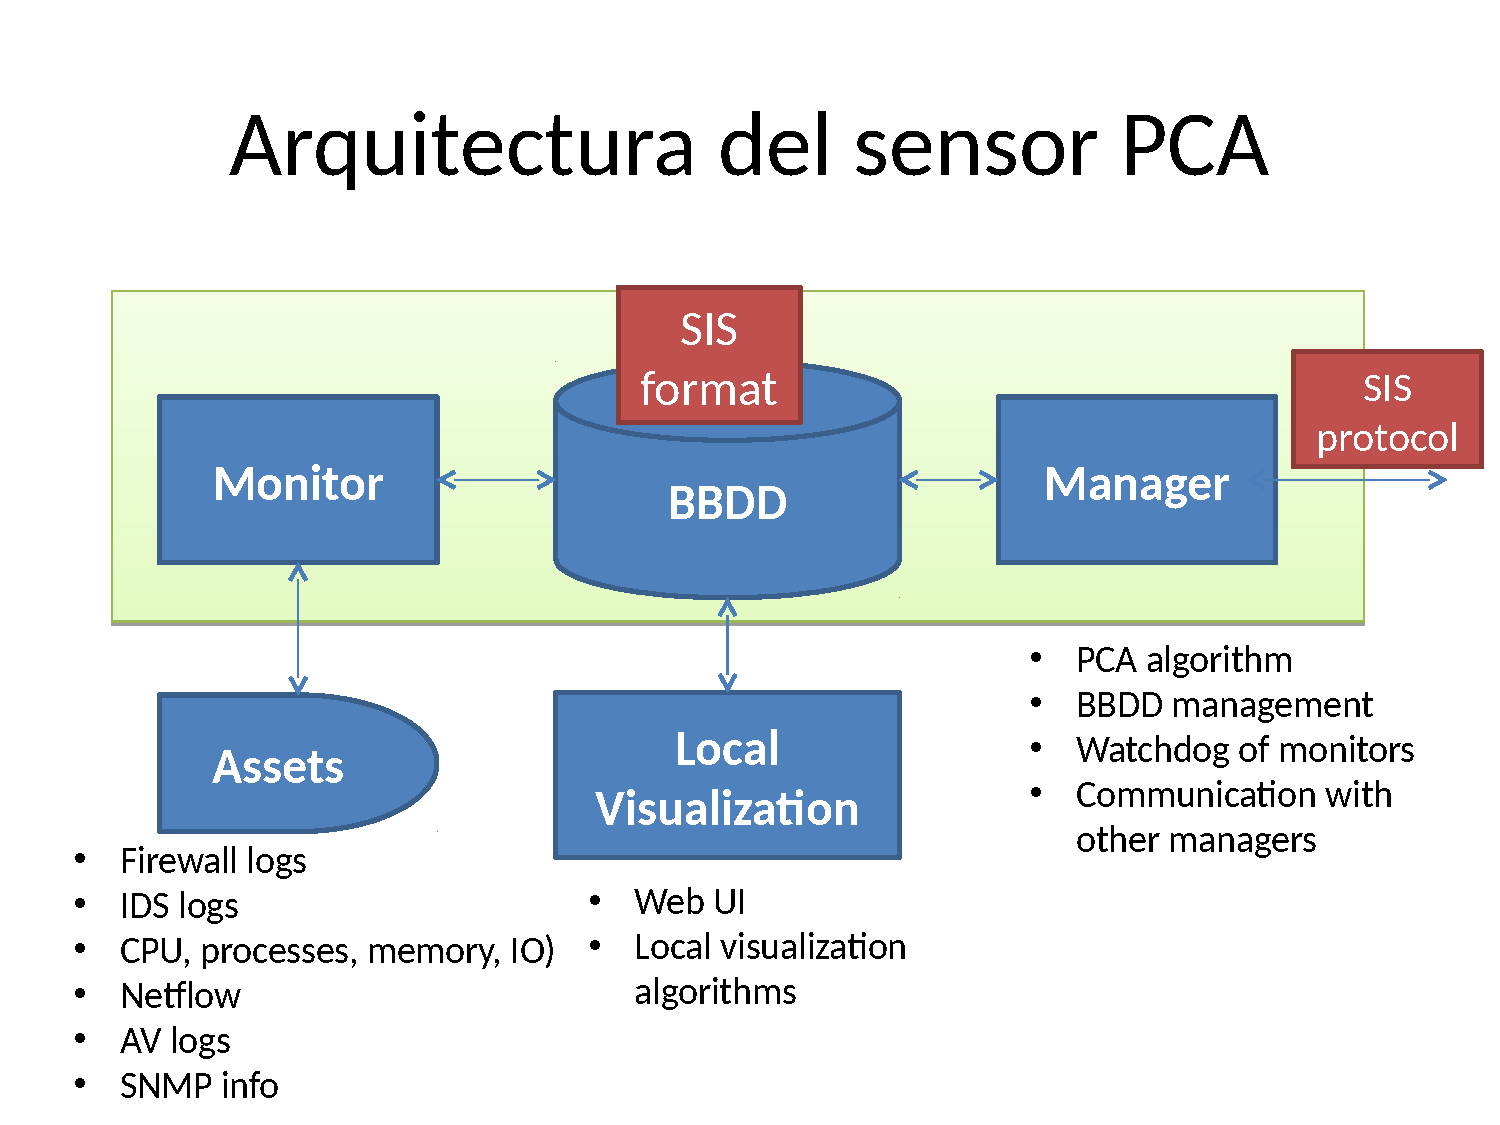
\includegraphics[scale=0.5]{diagramas/Especificaciones.pdf}}
  \caption{Arquitectura interna del software}
\end{figure}

\section{Visión global}

En cuanto a la estructura de esta memoria del proyecto final de carrera, tras éste capítulo dónde se presentan los objetivos y la visión en general del proyecto, se expone el estado del arte y el análisis de requisitos previos al desarrollo software.

En el capítulo siguiente, veremos la etapa del diseño de software así cómo posterior evaluación del mismo.

Finalmente, se presentan las conclusiones generales obtenidas una vez realizado el proyecto, así también la planifiación del mismo y estimación de costes.

Además, se presentan las referencia bibliográficas dónde se incluyen las fuentes consultadas para la elaboración de este proyecto, un resumen que engloba las generalidades fundamentales de la aplicación, una guía de utilización (manual de usuario), una guía de instalación, un compendio del software utilizado para el desarrollo y otro de los lenguajes de programación, y finalmente, la licencia completa del documento.
